
\chapter{Introduction and Background}

\section{Introduction}

% Context
This study is part of the broader context of the BugWright2 European project, which aims to solve the problem of autonomous inspection and maintenance of large metal structures with heterogeneous fleets of mobile robots.
In this project, we focus on the development of navigation strategies for a set of mobile robots using \gls{ugw}s, or Lamb waves, to perform the inspection of metal plates.
Indeed, guided waves have the particularity of propagating along a plate by interacting with the material that composes it, and by being affected by changes in geometry related, in particular, to corrosion.

% Problem definition
The main problem is therefore to define multi-robot navigation strategies to optimize the acquisition of data allowing to perform a tomography of metallic surfaces.
To achieve this objective, we will first carry out a bibliographical search, then set up navigation methods in a simulation environment.
Finally, we will consider deployment on different robots depending on the results obtained.
This project will be carried out under the supervision of Olivier Simonin (INSA Lyon CITI lab) and Cédric Pradalier (CNRS IRL2958 GT).

% Overview of Contributions
The expected contributions of this project are as follows:
\begin{itemize}
	\item Development of multi-robot navigation strategies for the acoustic inspection of metallic structures.
	\item Optimization of data acquisition for performing tomography.
	\item Resolution of coordination and synchronization issues between robots.
	\item Implementation of navigation methods in a simulation environment.
\end{itemize}

% Report Outline
This report presents the work carried out as part of my master's thesis on navigation and multi-robot control for the acoustic inspection of metal structures.
In the first section, we introduce the subject of the report, present the objectives of our project and describe the state of the art.
In the second section, we present the methodology used to carry out this project.
In the third section, we present the results obtained.
In the fourth section, we discuss the results obtained and the limitations of our work.
Finally, in the last section, we conclude on the work carried out and present the perspectives for future work.

\section{Preliminary Definitions}\label{sec:definitions}

Here, we will explain the preliminary assumptions and definitions that will be used in the remainder of this report.
First, we consider a planar environment, bounded and of known size.
We are not interested in the location of the robots in the environment, but we assume that each robot is able to know its position in the environment.
We also assume that the obstacles are localized in the environment.
Only the corrosion areas are not located.

We use \textit{crawler} robots. These robots are equipped with two drive wheels and an idler wheel.
An example crawler is shown in \ref{fig:crawler}.
The pose of the robot is defined by a triple $(x, y, \theta)$ where $x$ and $y$ are the coordinates of the robot in the environment and $\theta$ is the orientation of the robot in the environment.
We assume that the pose of the robot is known.
We also assume that the robots are able to synchronize in order to be able to move simultaneously or alternatively.
We note $cr$ the unit cost of rotation of the robot and $ct$ the unit cost of translation of the robot.

\begin{figure}[h!]
	\centering
	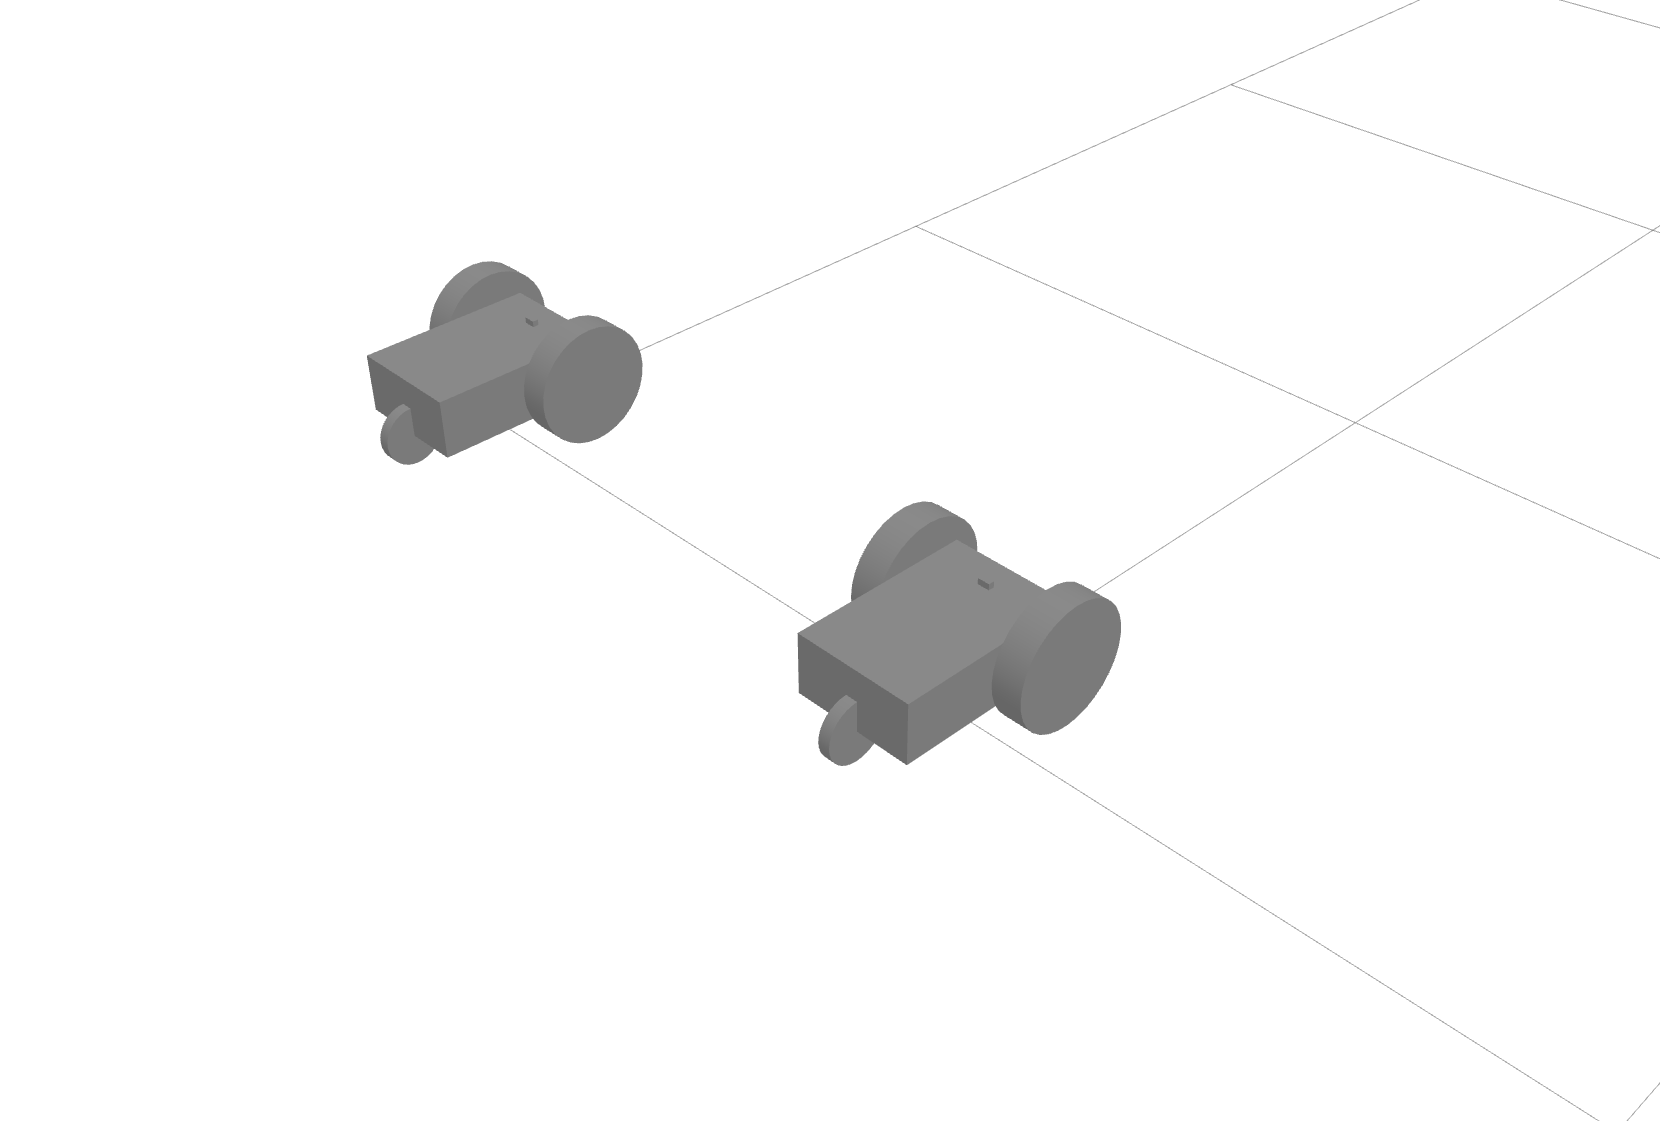
\includegraphics[width=0.5\textwidth]{graphics/crawlers.png}
	\caption{Crawler model used for acoustic inspection of metal structures.}
	\label{fig:crawler}
\end{figure}

Each robot is either a transmitter or a receiver, or both.
Crawlers are equipped with different sensors.
Among them :
\begin{itemize}
	\item an \gls{imu} sensor
	\item a piezoelectric or \gls{ugw} sensor
	\item a \gls{lidar} sensor
\end{itemize}
The \gls{imu} sensor makes it possible to know the orientation of the robot in the environment.
The \gls{ugw} sensor detects the presence of corrosion on the metal surface by emitting and receiving ultrasonic waves.
The \gls{lidar} sensor detects obstacles in the environment.
The obstacles considered here are mainly the various robots inspecting the metal surface.
Corrosion zones are detected by the emission of ultrasonic waves by a robot and the reception of these waves by another robot.
Insofar as the wave received by one of the crawlers is altered, then there is a point of corrosion between the transmitter robot and the receiver robot.
The detection of these corrosion zones is carried out in real time.
The maximum range of ultrasonic waves is noted $d_{max}$.
We approximate the propagation time of ultrasonic waves in the metal surface by zero time.

We use an occupancy grid to model the environment in which robots evolve during the acoustic inspection of metal structures.
This grid allows us to represent and categorize the different states of the areas of the metal surface.
The occupancy grid is composed of cells, where each cell corresponds to a small region of the environment.
In particular, we used a resolution of 0.05 meters per cell.
We use three states to characterize these cells: unknown, empty and occupied.
Unknown state refers to areas whose state has not yet been determined or detected.
The empty state indicates areas where there is no corrosion detected, i.e. the metal surface is sound.
Finally, the occupied state represents the identified corrosion areas, where the presence of defects or deterioration is detected.

By using this occupancy grid, we can track and update in real time the state of different areas of the metal surface during the inspection.
This allows us to plan robot movements, optimize their trajectory and ensure full coverage of the surface to be inspected.
In addition, this representation gives us a clear view of the state of corrosion of the metal structure, thus facilitating the analysis and evaluation of the results of the inspection.

In the rest of our proposal, we will detail the algorithms and methods used to update the occupancy grid according to the information collected by the robots' sensors.
We will also discuss multi-robot navigation strategies that leverage this modeling to optimize data acquisition and improve the efficiency of acoustic inspection.

\section{Background}

We present here the state of the art in the field of multi-robot navigation and control for the acoustic inspection of metal structures.
The objective of this literature review was to collect key information, analyze previous work and situate our project in the existing research context.
The references and sources cited in this section provide a solid foundation of knowledge and expertise on the subject.

Initially, we were interested in the properties of \gls{ugw}s and their applications in the field of tomography~\cite{OUABI2022106705, HUTHWAITE2013979}, mapping of robots and metallic structures~\cite{9364359, 9811581, inventions3030059, 9568841}, robots and sensors used in our project~\cite{s22093235}, multi-robot exploration~\cite{bautin:hal-00757960, articlesvsdf} as well as placement strategies for detection~\cite{article455556, 7487624, 7139673}.

In the paper~\cite{OUABI2022106705}, the authors propose a method to infer the geometry of metal plates using Lamb waves.
They use beamforming~\cite{enwiki:1151960654} to estimate plate boundaries based on acoustic measurements.
Experimental results show accurate inference of plate geometry.
However, the authors are content to map the contours of the structures, without proposing a method to map the defects, which is the subject of our problem.

The article~\cite{9364359} presents a FastSLAM-based approach~\cite{article254524} for robotic inspection of metal structures using ultrasound.
The authors propose a pioneer edge allocation method for multi-robot exploration, allowing fast and accurate inspection of structures.
Our work takes robot localization and mapping as known, and focuses on trajectory planning for the inspection of metal structures.
The approach used in this article can therefore be complementary to our work.

In the paper~\cite{9811581}, the authors propose a method for mapping metallic structures using \gls{ugw}s.
They combine a Cartesian grid with specific features for defect detection.
The experimental results show an accurate mapping of metallic structures.
However, the authors are once again content to map the outlines of the structures, without proposing a method for mapping the defects.

The article~\cite{inventions3030059} focuses on the localization of impacts in composite structures using a developed imaging method.
The authors use piezoelectric sensors~\cite{enwiki:1154129092} to detect and localize impacts, and a wavelet transform method~\cite{enwiki:1147185762} to analyze acoustic signals.
Experimental results show accurate detection and localization of impacts.
The sensors used are similar to those used in our project, but these sensors are positioned in a fixed way on the structure, while we want a mobile strategy.

In the paper~\cite{HUTHWAITE2013979}, the authors propose a high-resolution ultrasound tomography method for the quantification of wall thickness.
They exploit the dispersive nature of Lamb waves to convert variations in thickness into variations in wave velocity, thus enabling accurate reconstruction of wall thickness.
Experimental results show accurate reconstructions of corrosion defects.
This article was interesting to understand the properties of \gls{ugw}s and their applications in the field of tomography.

The article~\cite{s22093235}, resulting from the work of the BugWright2 project, presents a magnetic robot system for the inspection and autonomous maintenance of large structures.
The authors propose a localization framework based on a grid created from a point cloud, coupled with \gls{uwb} sensors and an \gls{imu}.
They also incorporate a piezoelectric sensor for \gls{ugw} detection for precise robot localization and structural feature mapping.
It is typically these robots and sensors that are used in our work.

The paper~\cite{bautin:hal-00757960} presents a planning algorithm for multi-robot exploration.
This algorithm, called \textit{MinPos}, is designed to efficiently allocate boundaries to robots in order to minimize the movement and time needed to explore the environment. It uses advanced optimization techniques to solve this problem effectively.
However, our work focuses on structural inspection for flaw detection.
We want a detailed inspection of corrosion areas and not a global exploration of the environment.

The article~\cite{article455556} presents strategies for the optimal placement of surveillance cameras in art galleries.
The authors propose methods to maximize surveillance coverage while minimizing the number of cameras needed.
However, the sensors used in our project are sensors that provide information on a segment only, between a transmitter and a receiver, and not global information like a camera.
The sensors used in our project are described in \ref{sec:definitions}.

In the article~\cite{articlesvsdf}, the authors propose a method for automatically locating and sizing defects in structures using guided wave imaging.
They use a convolutional neural network~\cite{enwiki:1159408824} to analyze guided wave signals and estimate defect sizes.
The experimental results show the efficiency of the proposed approach to invert both synthetic and experimental data.
This approach requires fixed sensors on the structure.
We want a mobile approach, not requiring the deployment of sensors on the structure.

The article~\cite{9568841} presents an autonomous on-plate exploration for an inspection robot using \gls{ugw}s.
The authors propose a localization method based on a mesh created from a cloud of points and use measurements from \gls{imu} and \gls{uwb} sensors.
They also integrate a piezoelectric sensor into the system for precise robot location and structural feature mapping.
In our approach, the location is assumed to be known.
This work can be used for robot localization, although this is not the subject of our project.
Nevertheless, the type of robot and sensors used are similar to those used in our project.

The article~\cite{7487624} presents effective measurement planning strategies for remote gas detection with mobile robots.
The objective of the study is to optimize the planning of measurements so as to maximize gas detection accuracy while minimizing the time and resources required.
The authors propose different approaches for planning measurements, including the use of exploration techniques based on the boundaries of detection zones, the selection of efficient trajectories to cover the environment and the reduction of the number of measurements necessary by using probabilistic models.
The type of sensor used has characteristics similar to those of the sensors used in our project.
However, our problem imposes movements of pairs of robots.
The way to split the investigation into two phases, a rough inspection phase and a refinement phase, is also similar to our approach.
However, this first phase is performed by fixed sensors, which is not desirable in our approach.
We will also use a \gls{tsp} to optimize robot movements between areas of interest.

In the paper~\cite{7139673}, the authors propose an efficient measurement planning method for remote gas detection with mobile robots.
Their approach is to optimize the planning of measures in order to minimize the time and resources required.
To do this, they use a convex relaxation technique in order to solve the optimization problem which allows to minimize the number of necessary measurements, while guaranteeing a complete coverage of the environment.
This study is interesting for our problem and could inspire improvements of our approach in the optimization of the \gls{tsp} used.

In summary, the works presented in this section are interesting for our problem, because they allowed us to deepen our knowledge of the problems related to guided wave tomography.
The articles~\cite{7487624, 7139673} are the closest to our problem.
However, these articles focus on covering the environment without worrying about the quality of the mapping of the areas of interest.
Moreover, these items use fixed sensors on the structure for the first rough inspection phase, which is not desirable in our approach.
This is why we propose a multi-robot navigation approach for the acoustic inspection of metallic structures in order to optimize the acquisition of data which will allow to carry out the tomography of metallic surfaces.

